%%%%%%%%%%%%%%%%%%%%%%%%%%%%%%%%%%%%%%%%%
% Diaz Essay
% LaTeX Template
% Version 2.0 (13/1/19)
%
% This template originates from:
% http://www.LaTeXTemplates.com
%
% Authors:
% Vel (vel@LaTeXTemplates.com)
% Nicolas Diaz (nsdiaz@uc.cl)
%
% License:
% CC BY-NC-SA 3.0 (http://creativecommons.org/licenses/by-nc-sa/3.0/)
%
%%%%%%%%%%%%%%%%%%%%%%%%%%%%%%%%%%%%%%%%%

%----------------------------------------------------------------------------------------
%	PACKAGES AND OTHER DOCUMENT CONFIGURATIONS
%----------------------------------------------------------------------------------------

\documentclass[9pt]{extarticle} % Font size (can be 10pt, 11pt or 12pt)
\usepackage{graphicx}
\usepackage[english]{babel}
\usepackage{geometry}
\setlength\parindent{0em}
\setlength{\parskip}{1em}
\usepackage{color}
\usepackage[cm]{fullpage}
\newcommand{\liam}[1]{\textcolor{red}{#1}}
%----------------------------------------------------------------------------------------
%	TITLE SECTION
%----------------------------------------------------------------------------------------

%\title{\textbf{Surviving the End of the World} \\ {\Large\itshape What to Do When Your Planet Is Destroyed}} % Title and subtitle

%\author{\textbf{Liam Sharp}\\ % Author and institution

%\date{\today} % Date, use \date{} for no date

%----------------------------------------------------------------------------------------

\begin{document}

%\maketitle % Print the title section

%----------------------------------------------------------------------------------------
%	ABSTRACT AND KEYWORDS
%----------------------------------------------------------------------------------------

%\renewcommand{\abstractname}{Summary} % Uncomment to change the name of the abstract to something else

\section*{Dissertation Abstract}
%%% REMOVE SEE FIG...
The nervous system has a unique diversity of lipids compared to any other mammalian cell \cite{Ingolfsson2014a}, containing $\sim 50\%$ saturated fatty acids, $\sim 20 \%$ $\omega$-3 polyunsaturated fatty acids (PUFAs) Figure \ref{fig:fig1} , and $\sim 35\%$ cholesterol per phospholipid \cite{Taguchi2010,Isolated1969,Breckenridge1973}. Decreased net concentrations of $\omega$-3 PUFAs have been shown to relate to, attention deficit disorder \cite{Manor2011}, bipolar disorder \cite{Koga2019}, severe depression \cite{Su2003}, and schizophrenia \cite{Maekawa2017} to name a few. In some cases ingesting $\omega$-3 rich foods and supplements (fish oil pills) has been shown to dramatically reduce symptoms \cite{DeFelice2012}. While the the role of $\omega$-3 PUFAs  neurological disorders is unknown, pLGIC are implicated in many of these disorders \cite{Xiong2012,Walstab2010,Picciotto_Neuroprotection_2008,MartinRuiz_4_1999,Haydar2010}.

pLGICs are a family of channels essential in synaptic function. pLGICs are known to be functionally dependent on their environment’s lipid composition \cite{Criado1984,Ellena1983,Fong1987,Jones1988,RyanSEDemersCNChewJP1996}. While the role of lipids is essential to pLGIC, the boundary lipids have not been identified in native or experimental membranes. In particular, the membranes of the most commonly used experimental systems (\textit{Xenopus} oocytes) have only one third the amount of $\omega$-3 fatty acids found in native membranes (Figure \ref{fig:fig1}).  The effect of the difference in bulk membrane composition on the local lipid environment of the nAChR (the boundary lipids) is unknown, but intrinsic nAChR lipid-sensitivity suggests non-native boundary lipids may introduce substantial artifacts in function.

It is experimentally unfeasible to visualize the individual boundary lipids surrounding membrane proteins. CG-MD simulations play the role of a ”computational microscope” to visualize lipid diffusion and various feasible lipid-protein arrangements in thermodynamically equilibrated systems over microseconds, allowing observations not readily seen experimentally. We have previously simulated the effect of $\omega$-3 PUFAs on the boundary effects of nAChR, predicting a preferential interaction with $\omega$-3 PUFAs and cholesterol \cite{Sharp2019,Woods2019}, two significant lipids in the post-synaptic membrane \cite{Taguchi2010,Isolated1969,Breckenridge1973}. We provide the first analysis of boundary lipid composition from simulations of nAChRs in neuronal and \textit{Xenopus} oocyte membranes. We find specific binding sites for $\omega$-3 PUFAs  in both membranes: pLGICs make a star-shape in the membrane, and omega-3 PUFAs bind at the tips of the star.  These sites are less likely to be occupied by $\omega$-3 PUFAs in the \textit{Xenopus} oocytes. 

%nAChR native membranes have approximately three times the $\omega$-3's PUFAs and one and a half times the cholesterol compared to \textit{Xenopus} oocytes \cite{Taguchi2010,Isolated1969,Breckenridge1973,Gamba2005}, see plots in Figure \ref{fig:fig2}; yet, $\omega$-3 PUFAs are infrequently used in pLGIC experimental studies.

It is unclear whether binding sites for PUFAs are determined by the particular amino acids around the binding site (the protein sequence) or the overall shape of the protein. While we predicted $\omega$-3 PUFAs interact favorably with nAChR, it is unknown if this hypothesis holds true for other pLGICs. The $\gamma$-aminobutyric acid type A receptor (GABA$_A$R), the serotonin receptor (5-HT3),  glutamate-gated chloride channels (GluCl) are eukaryotic pLGICs. Structures are conserved across pLGICs sequences \cite{Jaiteh2016}, but it is not know if sequence or structure determines boundary lipid composition. To differentiate the role of sequence vs. structure, we simulate a series of ternary membranes using saturated fatty acids,  $\omega$-6 PUFAs, and  $\omega$-3 PUFAs using various pLGICs with existing crystal or cryo-EM structures. We hypothesize one of two outcomes: 1) all pLGICs form a similar boundary distribution of PUFAs, suggesting lipid organization is a result of a shared structure. 2) Lipid distributions are dissimilar, and lipid organization is driven by protein sequence over the structure.


%----------------------------------------------------------------------------------------
%	ESSAY BODY
%----------------------------------------------------------------------------------------

\section*{Research Narrative}

%\subsection*{Neuronal Lipid Associated Diseases}

%Containing $\sim 50\%$ saturated fatty acids, $\sim 20 \%$ $\omega$-3 polyunsaturated fatty acids (PUFAs), and$\sim 35\%$ cholesterol per phospholipid, the nervous system has a unique diversity of lipids compared to any other cell line of mammalian physiology. Decreased net concentrations of $\omega$-3 PUFAs have been shown to relate to heightened anxiety, attention deficit disorder, bipolar disorder, sever depression, and schizophrenia to name a few. In all of these disorders ingesting $\omega$-3 rich foods and supplements (fish oil pills) has been shown to improve patients conditions.

%While the mechanism that relates $\omega$-3 PUFAs to neurological disorders is unknown, we have previously modeled the effect of $\omega$-3 PUFAs and the essential pentameric ligand gated ion channel (pLGIC) the nicotinic acetylcholine receptor (nAChR), predicting a structural dependence on $\omega$-3 PUFAs.


\subsection*{\textbf{Aim 1}: Nicotinic Acetylcholine Receptors Boundary Lipid Composition Within Simulated Coarse-Grained Native and Experimental Membranes}

There is a discernible difference between the boundary lipids of nAChR in neuronal and \textit{Xenopus} oocyte membranes. This work will predict what lipids need to be add to \textit{Xenopus} oocyte functional studies to mimic the nAChR's boundary lipids in neurons. Xenopus oocytes are used in ion channel functional studies \cite{Conti2013,Cornelison2016,Lee1994}; they are large single cells and easily manipulated. Due to the extreme lipid sensitivity of pLGICs, it is not clear that function in the experimental system reflects function in native membranes. However pLGICs do not reach native function without the inclusion of cholesterol \cite{Fong1987,Jones1988}, anionic lipids \cite{RyanSEDemersCNChewJP1996}, asolectin \cite{Fong1986,Fong1987}, or pLGIC native membrane \cite{Conti2013}. Comparing \textbf{neuronal membranes and \textit{Xenopus} oocytes} show \textbf{distinctly different} lipid compositions that have not been analyzed, see Figure \ref{fig:fig2}.  Of interest, many anionic lipids, asolectin, and native membranes are rich in polyunsaturated fatty acids. Combined with our previous prediction that nAChR has a high affinity for $\omega$-3 PUFAs, we hypothesize that nAChR requires substantial annular fraction PUFAs and cholesterol promote function, Figure 2. I have simulated neuronal and \textit{Xenopus} oocytes with one to three proteins using CG-MD for $10\mu s$. I am analyzing the boundary lipid interactions to determine what boundary lipids \textit{Xeonpus} oocytes need to mimic neuronal membranes.

\begin{figure}
    \center
    \includegraphics[width=.6\linewidth]{Lipid_doughnut.pdf}
    \caption{Side view of nAChR (left). Chemical structures of lipids (middle). Saturated fatty acid Steric Acid (top) and Docosahexaenoic acid (bottom). Lipid compositions (right) in an average mammalian cell (external), \textit{Xenopus} oocyte (middle), and a neuron (center) \cite{Taguchi2010,Isolated1969,Breckenridge1973,Ingolfsson2014a,Gamba2005}.}
    \label{fig:fig1}
\end{figure}



\subsection*{Aim 2: Is Boundary Lipid Composition Driven by Structure or Sequence}

 Determine the relative role pentameric ligand gated ion channel's sequence and structure play on boundary lipid composition. pLGIC sequence vary across species and even within individual species, despite all pLGICs having a conserved structure  Figure \ref{fig:fig3}. It is unclear whether boundary lipids organization is driven by a protein sequence or its structure. \textbf{We hypothesize the conserved structure promotes an affinity for long-chained PUFAs}\cite{Sharp2019,Woods2019}. If true, it would suggest all pLGICs have a similar affinity for flexible long chained $\omega$-3 PUFAs (diagramed in Figure \ref{fig:fig3}).

%\textit{Approach:} I am using CG-MD to simulate $\sim 5$ pLGICs in forty-four membrane compositions over $4\mu s$.
\begin{figure}
    \center
    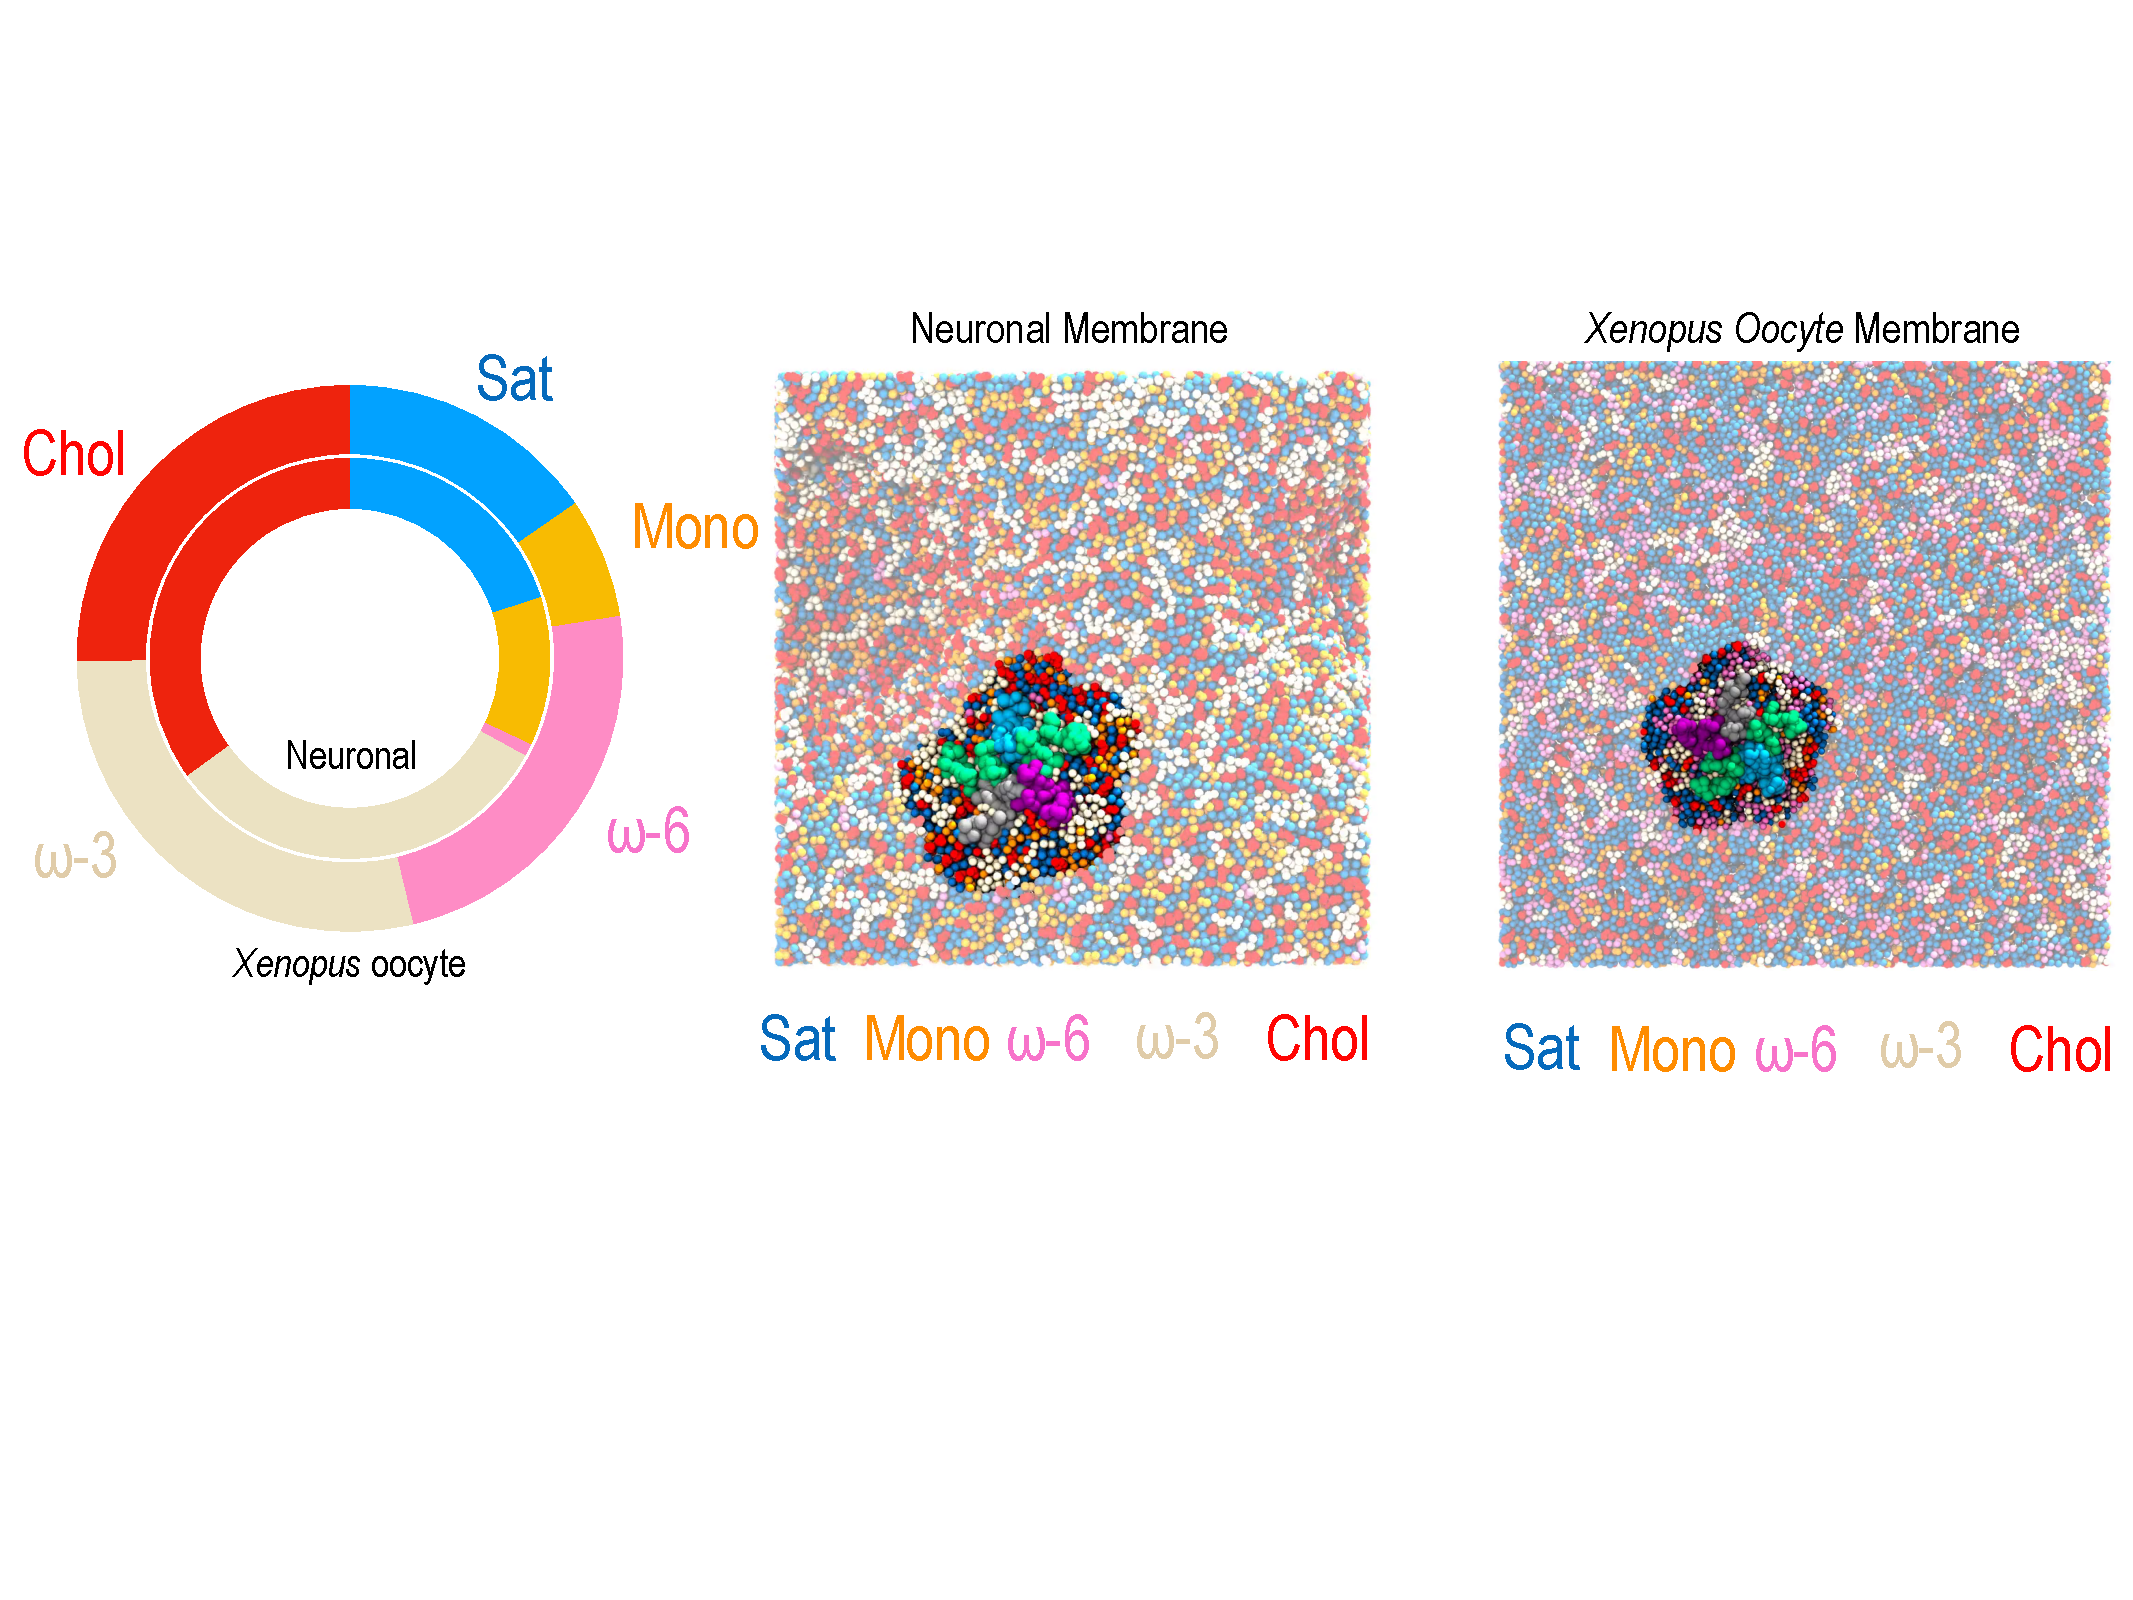
\includegraphics[width=.6\linewidth]{./Syn_Ooc.pdf}
    \caption{Boundary lipid fractions of nAChR (left) in neuronal (inner), and \textit{Xenopus} oocyte (external). nAChR embedded in neuronal and \textit{Xenopus} oocyte. Boundary lipids are highlighted (right).}
    \label{fig:fig2}
\end{figure}

%------------------------------------------------
\textit{Approach:} I am using CG-MD to simulate $\sim 5$ pLGICs in forty-four membrane compositions over $4\mu s$.
%\begin{figure}
    %\center
    %\includegraphics[width=.5\linewidth]{Heat_map_cartoon.pdf}
  %  \caption{Boundary lipid fractions of nAChR in neuronal (inner), and \textit{Xenopus} oocyte (external). nAChR %embedded in neuronal and \textit{Xenopus} oocyte. Boundary lipids are highlighted.}
%    \label{fig:fig2}
%\end{figure}

\begin{figure}
    \center
    \includegraphics[width=.5\linewidth]{Fig2.pdf}
    \caption{(Top) Three different pLGICs. While each has a different amino acid sequence they are structurally conserved. (Bottom) Cartoon representation of our hypothesis showing PUFA contact with PLGIC.}
    \label{fig:fig3}
\end{figure}

\section*{Effectiveness of the Award}
Being awarded this fellowship would alleviate financial stressors for the summer. My previous committee meeting agreed that I should submit Aim 1, and have Aim 2 near completion before defending. My advisor, Dr. Grace Brannigan, can fund me on a GA for 2020-2021 but cannot also afford summer funding.  This fellowship would cover my summer funding, allowing Dr Brannigan to fund me as a GA for 2020-2021. The alternative is that I would need to be a TA for my final year, which would slow down my progress substantially. 
%------------------------------------------------

\section*{Timeline to Completion}

\begin{itemize}
	\item April-May 2020: Complete simulations and analysis for Aim 1; Generate figures for Aim1; Complete simulations for Aim 2
	%\begin{itemize}
		%\item Complete simulations and analysis for Aim 1
		%\item Generate figures for Aim1
		%\item Complete simulations for Aim 2
	%\end{itemize}
	\item  \textit{June-July 2020}: Committee meeting; Write Aim 1 manuscript; Aim 2 Analysis; Generate figures for Aim 2
	%\begin{itemize}
	       % \item Committee meeting
		%\item Write Aim 1 manuscript
		%\item Aim 2 Analysis
		%\item Generate figures for Aim 2
	%\end{itemize}
	\item  \textit{August-September 2020}: Aim 1 manuscript submitted; Write Aim 2 Chapter
	%\begin{itemize}
      	%	\item Aim 1 manuscript submitted
       	% 	\item Write Aim 2 Chapter
	%\end{itemize}
	\item  \textit{October-November 2020}: Defend
	%\begin{itemize}
	%	\item Deffend
	%\end{itemize}
	\item \textit{December-January 2020-2021}: Graduate
	%\begin{itemize}
	%	\item Graduate
	%\end{itemize}
\end{itemize}

%----------------------------------------------------------------------------------------
%	BIBLIOGRAPHY
%----------------------------------------------------------------------------------------
\bibliographystyle{unsrt}
\bibliography{DisFellow}
%----------------------------------------------------------------------------------------

\end{document}
